\chapter{Index Analysis of the MNA}

der ane satz do + proof hopefully

seite 22 kap 7 netw top and dae ind for rlc - modelling and discretization circ prob

In the previous chapter we have seen two different kinds of Index concepts for differential algebraic equations. We have also seen that these two, even thoough they describe rather different structural aspects of the equation, are the same for our use-cases. This of course leads to the question : ``What are the indices we can usually expect for MNA?''.

This chapter aims to answer that question for the linear RLC case. Which means that the RLC components are described by linear functions with positive capacitances, inductances and resistances. Thus the matrices
\begin{displaymath}
	C:=\frac{\partial q_C(w)}{\partial w}, \quad L:=\frac{\partial \phi_L(w)}{\partial w}, \quad G:=\frac{\partial r(w)}{\partial w}
\end{displaymath}
are positive definite and symmetric.

The generalization of these results to the nonlinear case still relies on positive definiteness.

Recall that we consider the equations resulting from the analysis above. These equations are of the form \ref{DAE-const-coeff}
\begin{displaymath}
	A y'(t) + B y(t) = f(t).
\end{displaymath}
Specifically the obtained equations from the Modified Nodal Analysis \ref{MNA_Matrixform} are
\begin{displaymath}
	\begin{pmatrix}
		A_C C A_C^\top & 0 & 0 \\
		0 & L & 0 \\
		0 & 0 & 0
	\end{pmatrix}
	*
	\begin{pmatrix}
		\dot{u} \\
		\dot{i_L} \\
		\dot{i_V}
	\end{pmatrix}
	+
	\begin{pmatrix}
		A_R G A_R^\top & A_L & A_V \\
		-A_L^\top & 0 & 0 \\
		-A_V^\top & 0 & 0 ä
	\end{pmatrix}
	*
	\begin{pmatrix}
		u \\
		i_L \\
		i_V
	\end{pmatrix}
	=
	\begin{pmatrix}
		-A_I i_{src} \\
		0 \\
		-v_{src}
	\end{pmatrix}.
\end{displaymath}

\section{General Index analysis}

Assuming the system only contains linear elements or is linearized at an operating point in order to investigate the system behaviour then the corresponding network equation represents a DAE with constant coefficients \ref{DAE-const-coeff}. We will denote $x=(u, i_L, i_V)^\top$. The structure of the system is reliant on the matrix $B$, thus we consider

\begin{itemize}
	\item \textbf{ODE-case}: \newline
	The matrix $B$ is regular in \ref{DAE-const-coeff}. This is the case iff the circuit contains no voltage sources and there are no nodes which have no path to ground via capacitors. Then the system represents a linear-implicit system of ODEs and can be transformed into the explicit ODE sytstem
	\begin{displaymath}
		\dot{x}=B^{-1}(-Ax+f(t)).
	\end{displaymath}
	Thus we obtain an index of $0$.
		
	\item \textbf{DAE-case}:
	The matrix $B$ is singular in \ref{DAE-const-coeff}. This is the interesting case which we will analyse further.
\end{itemize}

For the matrix $B$ being singular we have already obtained a representation of the form
\begin{align*}
	u'(t) + Ru(t) &= s(t), \\
	Nv'(t) + v(t) &= q(t)
\end{align*}
in the previous chapter. We now consider the nilpotency index of the matrix $N$, we already know that this index correlates with the differentiation as well as the perturbation index. We consider two cases:

\begin{enumerate}
	\item \textbf{The nilpotency index is 1} \newline
		Because $N$ is nilpotent with nipotency index $\nu = 1$ it holds that $N^1 = 0$, thus the system transforms to
		\begin{align*}
			u'(t) + Ru(t) &= s(t), \\
			v(t) &= q(t).
		\end{align*}
		This means that the algebraic variables are given explicitly. Thus the system can be written in ODE form. (what properies does R have? - state ODE form)

	\item \textbf{The nilpotency index is $\geq$ 2} \newline
		This case is the situation we have seen in \ref{Weierstraß-Kronecker Normalform} , it led to \ref{solution-to-transformed-DAE-const-coeff-part2}
		\begin{displaymath}
			v(t) = \sum_{i=0}^{k-1} (-1)^iN^iq^{(i)}(t).
		\end{displaymath}
		By differentiating one more time we receive
		\begin{equation}
			v'(t) = \sum_{i=0}^{k-1} (-1)^iN^iq^{(i+1)}(t)
		\end{equation}
		with the assumption that $q$ is $\nu$ times differentiable.
\end{enumerate}

We can see that an algebraic constraint has to be fulfilled by the solution. In the case of index 1 this equation is given explicitly, for index $\geq$ 2 it is given implicitly.

The system is also sensitive to perturbations. Small noise in the input can have arbitrarily large derivatives which can influence $v$ as we it depends on them.

Thus no severe numerical problems arise from index-1 systems. Hence implicit numerical integration schemes for stiff systems are feasable. On the other hand severe nunmerical problems may occur in the case that the system has index greater or equal to $2$. The hidden constraints can only be resolved by an unstable differentiation process.

As $\nu$ defines the behaviour of the system theoretically as well as numerically it is called the \emph{algebraic index} of the linear implicit system.



\begin{figure}[H]
	\centering
	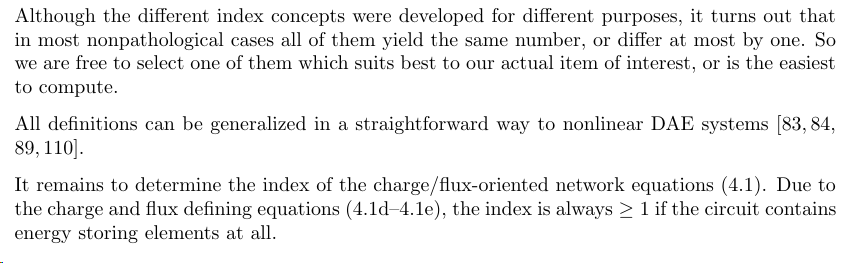
\includegraphics[width=0.7\linewidth]{screenshot022}
	\caption{}
	\label{fig:screenshot022}
\end{figure}


\section{Topological Conditions} 
reference to Tischendorf
basically chapter 7 of modelling book

From analyzing the MNA some conditions to the circuit topology can be obtained. We will be considering the impact of special arrangements of components on the index of the system. In \cite{Tischendorf2005Topological} they present very interesting results about the index of MNA equations.


\begin{theorem}[Index-1 condition] \cite{Tischendorf2004Topological}
	Let the matrices of the capacitances, inductances and resistances respectively be positive definite. If the network neither cointains \emph{inductance-current-source cutsets} nor (controlled?) \emph{capacitance-voltage-source loops}, then the MNA leads to an index-1 DAE.
\end{theorem}

Where inductance-current-source cutsets and capacitance-voltage-source loops are subcircuits of the form Seite 481 (searchbar) in basic circuit theory

\begin{figure}[H]
	\label{cutset and loop}
	\begin{subfigure}{0.5\textwidth}
		\centering
		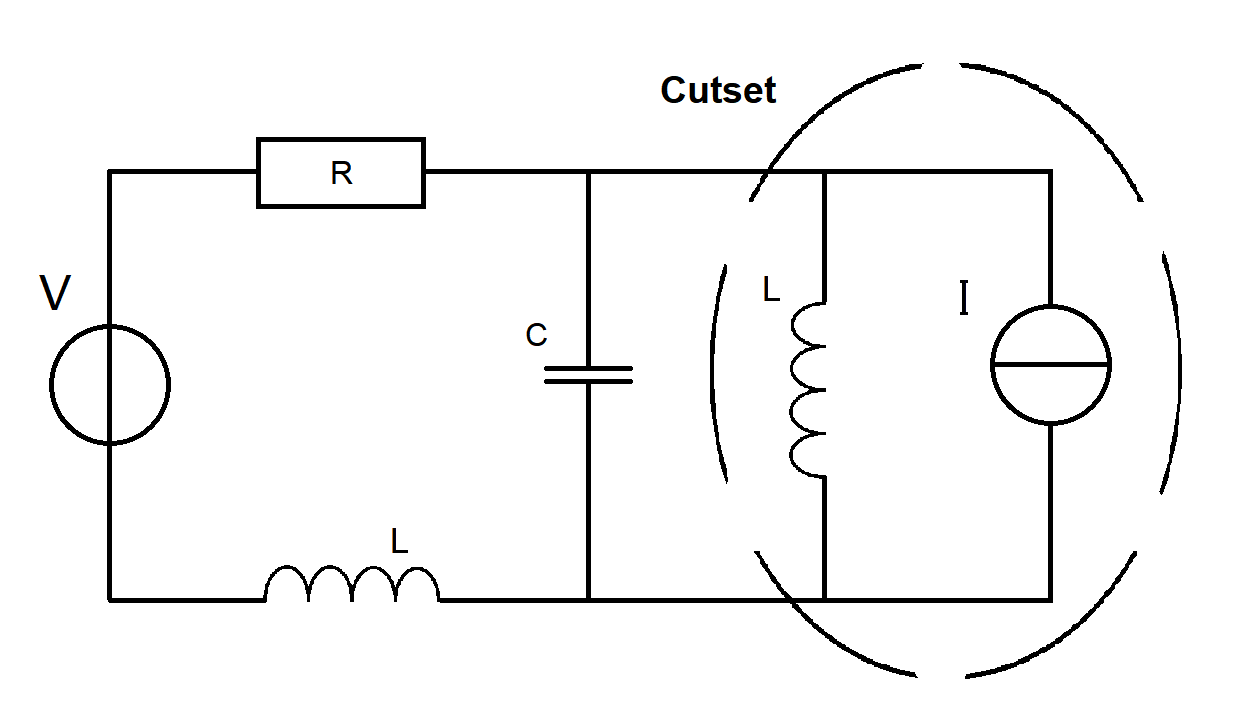
\includegraphics[width=0.9\linewidth]{pictures/inductance-current-source_cutset.png}
		\caption{inductance-current-source cutset}
	\end{subfigure}
	\begin{subfigure}{0.5\textwidth}
		\centering
		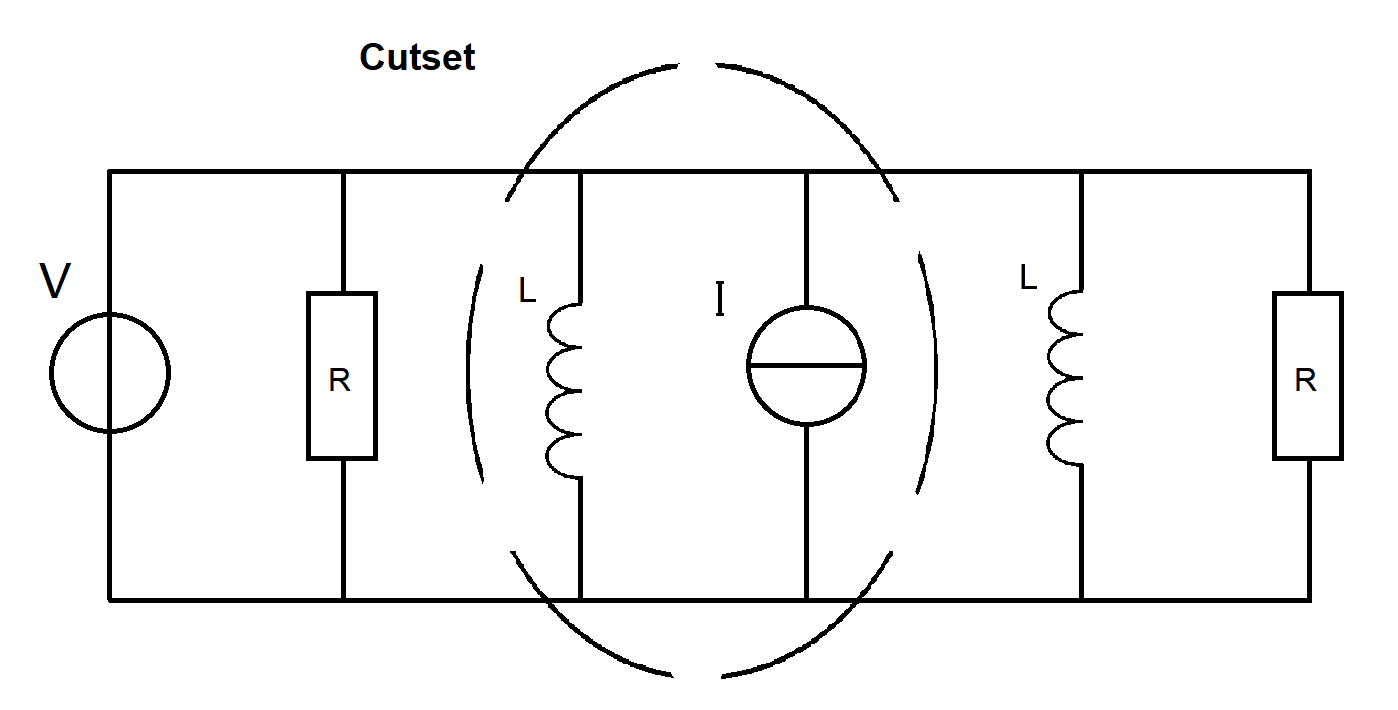
\includegraphics[width=0.9\linewidth]{pictures/capacitance-voltage-source_loop.png}
		\caption{capacitance-voltage-source loop}
	\end{subfigure}
\end{figure}

This means that if our circuit does not contain any loops or cutsets of the above form the resulting MNA has index 1.

\begin{theorem}[Index-2 condition] \cite{Tischendorf2004Topological}
	If the Network contains \emph{inductance-current-source cutsets} or \emph{capacitance-voltage-source loops} except for capacitance-only loops, then the MNA leads to an index-2 DAE.
\end{theorem}




This means that for ``reasonable'' RLC circuits (satisfying the prerequisites from the above theorems) the index will not exceed 2.

These results can also be interpreted in a more formal way. As they are just descriptions of the topology of the circuit we can reformulate the theorems in terms of the incidence matrix $A$.

ker conditions from page 22 - kapitel 7 quasi

WE will apply those results to some examples: